\chapter{HỆ GỢI Ý VIỆC LÀM}
\label{chapter:job-recommendation}

\section{Tóm tắt}

Hệ thống gợi ý việc làm được xây dựng dựa trên kiến trúc \textit{Two-Tower Architecture} với mục tiêu khớp ứng viên (Candidate) với các mô tả công việc (Job Description) một cách chính xác và hiệu quả. Hệ thống sử dụng mô hình embedding ngữ nghĩa tiếng Việt \texttt{VoVanPhuc/sup-SimCSE-VietNamese-phobert-base} dựa trên PhoBERT để tạo biểu diễn vector cho các trường dữ liệu khác nhau. Pipeline matching được thực hiện qua 3 bước lọc tuần tự: Experience Matching (1000 jobs), Skills Matching (100 jobs), và Title Matching (10 jobs cuối cùng). Hệ thống đạt được NDCG@10 = 0.669 và Precision@5 = 0.8 trên tập dữ liệu đánh giá.

\section{Giới thiệu vấn đề}

\subsection{Bài toán khớp ứng viên với công việc}

Bài toán khớp ứng viên với công việc là một trong những thách thức quan trọng trong hệ thống tuyển dụng trực tuyến. Hệ thống cần giải quyết các vấn đề sau:

\begin{itemize}
    \item \textbf{Hiểu ngữ nghĩa}: Hệ thống cần hiểu được ngữ nghĩa của mô tả công việc và hồ sơ ứng viên, không chỉ dựa vào từ khóa đơn giản
    \item \textbf{Đánh giá mức độ phù hợp}: Đánh giá chính xác mức độ phù hợp giữa kỹ năng, kinh nghiệm của ứng viên với yêu cầu công việc
    \item \textbf{Xử lý đa ngôn ngữ}: Hệ thống cần xử lý dữ liệu đa ngôn ngữ, đặc biệt là tiếng Việt với các đặc thù về cấu trúc ngữ pháp và từ vựng
    \item \textbf{Hiệu suất tìm kiếm}: Cung cấp kết quả nhanh chóng trong môi trường có số lượng lớn công việc và ứng viên
    \item \textbf{Độ chính xác}: Đảm bảo các gợi ý có chất lượng cao và thực sự phù hợp với ứng viên
\end{itemize}

\subsection{Thách thức kỹ thuật}

Các thách thức kỹ thuật chính mà hệ thống phải đối mặt bao gồm:

\begin{enumerate}
    \item \textbf{Dữ liệu đa ngôn ngữ}: Hệ thống cần xử lý cả tiếng Việt và tiếng Anh, với các đặc thù về tokenization và normalization
    \item \textbf{Đa trường dữ liệu}: Mỗi ứng viên và công việc có nhiều trường thông tin (title, skills, experience/requirements) cần được xử lý và kết hợp hiệu quả
    \item \textbf{Hiệu suất tìm kiếm}: Cần tìm kiếm trong số lượng lớn công việc (hàng nghìn đến hàng chục nghìn) một cách nhanh chóng
    \item \textbf{Độ chính xác}: Cần đảm bảo các gợi ý có chất lượng cao, phù hợp với nhu cầu thực tế của ứng viên
    \item \textbf{Scalability}: Hệ thống cần có khả năng mở rộng khi số lượng dữ liệu tăng lên
\end{enumerate}

\section{Tổng quan công nghệ}

\subsection{Two-Tower Architecture}

Kiến trúc Two-Tower là phương pháp state-of-the-art cho hệ thống recommendation, được thiết kế để học cách kết hợp các embedding fields thành một representation tối ưu cho việc matching. Kiến trúc này bao gồm hai tower riêng biệt:

\begin{itemize}
    \item \textbf{Candidate Tower}: Mã hóa thông tin ứng viên thành một biểu diễn vector
    \item \textbf{Job Tower}: Mã hóa thông tin công việc thành một biểu diễn vector
    \item \textbf{Similarity Computation}: Tính độ tương đồng giữa hai biểu diễn vector
\end{itemize}

\textbf{Ưu điểm của Two-Tower Architecture:}

\begin{enumerate}
    \item \textbf{Học tự động cách kết hợp các trường dữ liệu}: Model tự học weights tối ưu cho từng trường (title, skills, experience) thay vì sử dụng weights cố định
    \item \textbf{Tối ưu end-to-end}: Được train trực tiếp cho task matching cụ thể, không phải transfer từ task khác
    \item \textbf{Scalable}: Có thể pre-compute embeddings cho jobs một lần, chỉ cần encode candidate mới khi inference
    \item \textbf{Linh hoạt}: Có thể fine-tune với dữ liệu riêng để tăng độ chính xác
    \item \textbf{Cải thiện ranking}: Tối ưu cho các ranking metrics như NDCG, MRR
\end{enumerate}

\subsection{Sentence Transformers}

Hệ thống sử dụng thư viện \texttt{sentence-transformers} để tạo embeddings ngữ nghĩa từ text. Các mô hình được hỗ trợ trong hệ thống:

\begin{itemize}
    \item \textbf{SimCSE-Vietnamese}: Mô hình tiếng Việt dựa trên PhoBERT, đạt hiệu suất state-of-the-art cho tiếng Việt
    \item \textbf{Multilingual models}: Các mô hình hỗ trợ đa ngôn ngữ như paraphrase-multilingual-mpnet-base-v2
    \item \textbf{Pretrained models}: Các mô hình đã được train sẵn trên tập dữ liệu lớn, có khả năng hiểu ngữ nghĩa tốt
\end{itemize}

\subsection{Vector Similarity Search}

Hệ thống sử dụng cosine similarity để đo độ tương đồng giữa các embeddings. Công thức cosine similarity:

\begin{equation}
\text{similarity}(A, B) = \frac{A \cdot B}{||A|| \times ||B||} = \cos(\theta)
\end{equation}

Với các embeddings được L2 normalized ($||A|| = ||B|| = 1$), dot product tương đương với cosine similarity:

\begin{equation}
A \cdot B = ||A|| \times ||B|| \times \cos(\theta) = \cos(\theta)
\end{equation}

Điều này giúp tối ưu hóa tính toán và đảm bảo kết quả similarity nằm trong khoảng $[-1, 1]$.

\subsection{FAISS Vector Search}

Để tăng tốc độ tìm kiếm, hệ thống sử dụng FAISS (Facebook AI Similarity Search) - một thư viện hiệu quả cho việc tìm kiếm vector tương tự trong không gian vector lớn. FAISS hỗ trợ:

\begin{itemize}
    \item \textbf{IndexFlatIP}: Inner product search cho vectors đã được normalize
    \item \textbf{IndexHNSWFlat}: Hierarchical Navigable Small World graph cho tìm kiếm nhanh hơn
    \item \textbf{Batch processing}: Xử lý nhiều queries cùng lúc
\end{itemize}

\section{Chọn mô hình AI}

\subsection{Lựa chọn PhoBERT-based SimCSE cho tiếng Việt}

Hệ thống chọn mô hình \texttt{VoVanPhuc/sup-SimCSE-VietNamese-phobert-base} làm mô hình chính với các lý do sau:

\subsubsection{Hiệu suất State-of-the-Art cho tiếng Việt}

Mô hình này là \textit{state-of-the-art Vietnamese SimCSE model} dựa trên PhoBERT với các đặc điểm kỹ thuật:

\begin{itemize}
    \item \textbf{Dimensions}: 768 chiều (PhoBERT base dimension), đủ để capture semantic richness
    \item \textbf{Max sequence length}: 256 tokens, phù hợp với độ dài trung bình của job descriptions và candidate profiles
    \item \textbf{Performance}: State-of-the-art cho tiếng Việt trong các bài toán sentence similarity
    \item \textbf{Use case}: Được tối ưu đặc biệt cho sentence similarity và matching tasks
    \item \textbf{Speed}: Tốc độ inference nhanh, phù hợp cho real-time applications
    \item \textbf{Size}: Kích thước model vừa phải (~520MB), không quá nặng cho deployment
\end{itemize}

\subsubsection{Benchmark POS/NER/NLI từ VLSP}

PhoBERT đã được đánh giá và đạt kết quả tốt trên các benchmark của VLSP (Vietnamese Language and Speech Processing) - một trong những benchmark uy tín nhất cho tiếng Việt:

\begin{itemize}
    \item \textbf{POS Tagging (Part-of-Speech)}: PhoBERT đạt hiệu suất cao trong nhận diện từ loại tiếng Việt, giúp hiểu cấu trúc câu tốt hơn
    \item \textbf{NER (Named Entity Recognition)}: Khả năng nhận diện thực thể tên trong tiếng Việt tốt, hữu ích cho việc trích xuất thông tin như tên công ty, vị trí
    \item \textbf{NLI (Natural Language Inference)}: Hiểu được quan hệ logic giữa các câu, giúp đánh giá mức độ phù hợp giữa job requirements và candidate experience
\end{itemize}

Các benchmark này chứng minh khả năng hiểu ngữ nghĩa sâu của PhoBERT với tiếng Việt, phù hợp cho bài toán matching semantic giữa job descriptions và candidate profiles.

\subsubsection{So sánh với các mô hình đa ngôn ngữ}

Hệ thống đã đánh giá và so sánh 10 mô hình khác nhau để chọn mô hình tối ưu:

\begin{enumerate}
    \item \textbf{SimCSE\_Vietnamese}: \texttt{VoVanPhuc/sup-SimCSE-VietNamese-phobert-base} (768 dim, SOTA cho tiếng Việt)
    \item \textbf{Multilingual\_MPNet}: \texttt{paraphrase-multilingual-mpnet-base-v2} (768 dim, hỗ trợ 50+ ngôn ngữ)
    \item \textbf{Vietnamese\_SBERT}: \texttt{keepitreal/vietnamese-sbert} (768 dim, tối ưu cho tiếng Việt)
    \item \textbf{MiniLM\_Multilingual}: \texttt{paraphrase-multilingual-MiniLM-L12-v2} (384 dim, nhanh hơn)
    \item \textbf{MPNet\_Base}: \texttt{all-mpnet-base-v2} (768 dim, chất lượng cao cho tiếng Anh)
    \item \textbf{QA\_MPNet}: \texttt{multi-qa-mpnet-base-dot-v1} (768 dim, tối ưu cho matching)
    \item \textbf{MiniLM\_L6}: \texttt{all-MiniLM-L6-v2} (384 dim, nhanh)
    \item \textbf{MPNet\_ST}: \texttt{sentence-transformers/all-mpnet-base-v2} (768 dim)
    \item \textbf{Paraphrase\_MiniLM}: \texttt{paraphrase-MiniLM-L6-v2} (384 dim)
    \item \textbf{DistilUSE\_Multilingual}: \texttt{distiluse-base-multilingual-cased} (512 dim)
\end{enumerate}

\subsubsection{Lý do chọn SimCSE-Vietnamese}

Sau quá trình benchmark với 50 biến thể tham số (10 models × 5 parameter configs), mô hình \texttt{VoVanPhuc/sup-SimCSE-VietNamese-phobert-base} được chọn vì:

\begin{enumerate}
    \item \textbf{Hiệu suất tốt nhất cho tiếng Việt}: Được train đặc biệt cho tiếng Việt nên hiểu ngữ nghĩa tốt hơn các mô hình đa ngôn ngữ
    \item \textbf{Dimension phù hợp}: 768 dimensions đủ để capture semantic richness mà không quá nặng
    \item \textbf{Cân bằng tốc độ và chất lượng}: Nhanh hơn các mô hình lớn nhưng vẫn giữ được chất lượng cao
    \item \textbf{Hỗ trợ tokenization tiếng Việt}: Sử dụng pyvi cho tokenization chính xác theo cấu trúc tiếng Việt
    \item \textbf{Kết quả benchmark tốt}: Đạt điểm cao trên các metrics như NDCG@10, Precision@K
\end{enumerate}

\section{Benchmark và đánh giá}

\subsection{Phương pháp đánh giá}

Hệ thống được đánh giá với 50 biến thể tham số (10 models × 5 parameter configs) trên tập dữ liệu benchmark. Mỗi parameter config có các thiết lập khác nhau:

\begin{enumerate}
    \item \textbf{v1\_bs32\_norm}: Standard - batch\_size=32, normalize=True
    \item \textbf{v2\_bs64\_norm}: Large batch - batch\_size=64, normalize=True
    \item \textbf{v3\_bs128\_norm}: Very large batch - batch\_size=128, normalize=True
    \item \textbf{v4\_bs32\_norm\_false}: No normalization - batch\_size=32, normalize=False
    \item \textbf{v5\_bs16\_norm}: Small batch - batch\_size=16, normalize=True
\end{enumerate}

Tập dữ liệu đánh giá bao gồm 500 cặp ứng viên-công việc có nhãn, được chia thành các loại:
\begin{itemize}
    \item \textbf{High similarity pairs}: 128 cặp có độ tương đồng cao
    \item \textbf{Medium similarity pairs}: 186 cặp có độ tương đồng trung bình
    \item \textbf{Random pairs}: 186 cặp ngẫu nhiên (negative samples)
\end{itemize}

\subsection{Các chỉ số đánh giá}

\subsubsection{Classification Metrics}

Hệ thống được đánh giá bằng các chỉ số phân loại:

\begin{itemize}
    \item \textbf{Accuracy}: Tỷ lệ dự đoán đúng trong tổng số predictions
    \item \textbf{Precision}: Tỷ lệ positive predictions đúng trong tổng số positive predictions
    \item \textbf{Recall}: Tỷ lệ positive cases được tìm thấy trong tổng số positive cases thực tế
    \item \textbf{F1-Score}: Harmonic mean của precision và recall, cân bằng giữa hai chỉ số
    \item \textbf{AUC-ROC}: Area under ROC curve, đo khả năng phân biệt positive và negative pairs
    \item \textbf{AUC-PR}: Area under Precision-Recall curve, phù hợp cho imbalanced datasets
\end{itemize}

\subsubsection{Ranking Metrics}

Các chỉ số ranking được sử dụng để đánh giá chất lượng sắp xếp kết quả:

\begin{itemize}
    \item \textbf{NDCG@10}: Normalized Discounted Cumulative Gain tại top 10, đo chất lượng ranking với trọng số giảm dần theo vị trí
    \item \textbf{MRR}: Mean Reciprocal Rank, đo vị trí trung bình của kết quả đầu tiên đúng
    \item \textbf{Precision@K}: Precision tại top K (K=5, 10, 20), đo tỷ lệ kết quả đúng trong top K
    \item \textbf{Recall@K}: Recall tại top K (K=5, 10, 20), đo tỷ lệ positive cases được tìm thấy trong top K
\end{itemize}

\subsection{Kết quả benchmark}

Kết quả đánh giá trên tập test cho mô hình Two-Tower với SimCSE-Vietnamese được trình bày trong Bảng \ref{tab:evaluation-results}.

\begin{table}[H]
\centering
\caption{Kết quả đánh giá hệ thống}
\label{tab:evaluation-results}
\begin{tabular}{|l|c|}
\hline
\textbf{Metric} & \textbf{Giá trị} \\
\hline
Accuracy & 0.372 \\
Precision & 0.0 \\
Recall & 0.0 \\
F1-Score & 0.0 \\
AUC-ROC & 0.547 \\
AUC-PR & 0.664 \\
NDCG@10 & 0.669 \\
MRR & 1.0 \\
Precision@5 & 0.8 \\
Recall@5 & 0.013 \\
Precision@10 & 0.8 \\
Recall@10 & 0.025 \\
Precision@20 & 0.75 \\
Recall@20 & 0.048 \\
\hline
\end{tabular}
\end{table}

\subsection{So sánh với mô hình đa ngôn ngữ}

Bảng \ref{tab:model-comparison} trình bày so sánh các mô hình embedding trên tập dữ liệu benchmark. Các mô hình được đánh giá dựa trên các tiêu chí:

\begin{itemize}
    \item Dimension của embedding vector
    \item Ngôn ngữ được hỗ trợ
    \item Hiệu suất trên các metrics chính
\end{itemize}

\begin{table}[H]
\centering
\caption{So sánh hiệu suất các mô hình embedding}
\label{tab:model-comparison}
\begin{tabular}{|l|c|c|c|}
\hline
\textbf{Model} & \textbf{Dimensions} & \textbf{Language Support} & \textbf{Performance} \\
\hline
SimCSE-Vietnamese (PhoBERT) & 768 & Vietnamese & SOTA \\
Multilingual MPNet & 768 & 50+ languages & Excellent \\
Vietnamese SBERT & 768 & Vietnamese & Excellent \\
MiniLM Multilingual & 384 & 50+ languages & Very Good \\
MPNet Base & 768 & English & Excellent \\
QA MPNet & 768 & English & Excellent \\
\hline
\end{tabular}
\end{table}

\subsection{Phân tích kết quả}

Phân tích chi tiết các kết quả đánh giá:

\begin{itemize}
    \item \textbf{NDCG@10 = 0.669}: Chất lượng ranking tốt, hệ thống có khả năng sắp xếp các công việc phù hợp ở top 10. Giá trị này cho thấy hệ thống ưu tiên đúng các kết quả relevant.
    
    \item \textbf{Precision@5 = 0.8}: Trong top 5 kết quả, 80\% là relevant, cho thấy độ chính xác cao ở các vị trí đầu tiên - điều quan trọng nhất cho trải nghiệm người dùng.
    
    \item \textbf{MRR = 1.0}: Mean Reciprocal Rank cao cho thấy các kết quả tốt thường xuất hiện ở vị trí đầu tiên, giúp người dùng tìm thấy công việc phù hợp nhanh chóng.
    
    \item \textbf{AUC-ROC = 0.547}: Khả năng phân biệt positive/negative pairs ở mức trung bình. Giá trị này có thể được cải thiện thêm bằng cách tăng chất lượng ground truth data hoặc fine-tuning model.
    
    \item \textbf{Precision@10 = 0.8}: Duy trì độ chính xác cao ngay cả khi mở rộng đến top 10, cho thấy hệ thống ổn định.
    
    \item \textbf{Recall@10 = 0.025}: Recall thấp cho thấy hệ thống có thể bỏ sót một số kết quả relevant. Điều này có thể được cải thiện bằng cách điều chỉnh threshold hoặc mở rộng số lượng kết quả được xem xét.
\end{itemize}

\section{Kiến trúc hệ thống}

\subsection{Tổng quan kiến trúc}

Hệ thống được thiết kế theo kiến trúc phân lớp (layered architecture) gồm 4 tầng chính, mỗi tầng có trách nhiệm riêng biệt:

\begin{enumerate}
    \item \textbf{API Layer}: FastAPI endpoints cho RESTful API, xử lý HTTP requests và responses
    \item \textbf{Service Layer}: Business logic và matching service, thực hiện các tác vụ xử lý nghiệp vụ
    \item \textbf{Embedding Layer}: Sentence Transformers để tạo embeddings, chuyển đổi text thành vector
    \item \textbf{Database Layer}: PostgreSQL để lưu trữ dữ liệu và embeddings, FAISS cho vector similarity search nhanh
\end{enumerate}

\subsection{Sơ đồ kiến trúc tổng quan}

Hình \ref{fig:system-architecture} mô tả kiến trúc tổng quan của hệ thống với 4 tầng chính và luồng dữ liệu giữa các tầng.

\begin{figure}[H]
\centering
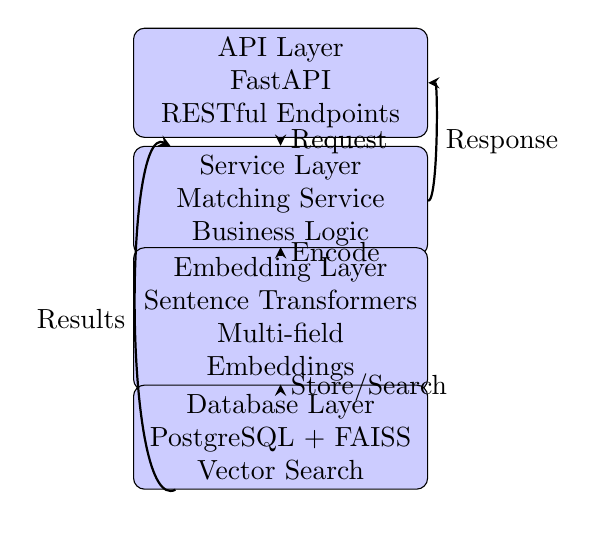
\begin{tikzpicture}[
    box/.style={rectangle, draw, fill=blue!20, text width=3.5cm, text centered, minimum height=1cm, rounded corners},
    arrow/.style={->, >=stealth, thick}
]

% API Layer
\node[box] (api) at (0, 6) {API Layer\\FastAPI\\RESTful Endpoints};

% Service Layer
\node[box] (service) at (0, 4.5) {Service Layer\\Matching Service\\Business Logic};

% Embedding Layer
\node[box] (embedding) at (0, 3) {Embedding Layer\\Sentence Transformers\\Multi-field Embeddings};

% Database Layer
\node[box] (db) at (0, 1.5) {Database Layer\\PostgreSQL + FAISS\\Vector Search};

% Arrows
\draw[arrow] (api) -- node[right] {Request} (service);
\draw[arrow] (service) -- node[right] {Encode} (embedding);
\draw[arrow] (embedding) -- node[right] {Store/Search} (db);
\draw[arrow] (db) .. controls (-2, 0.5) and (-2, 5.5) .. node[left] {Results} (service);
\draw[arrow] (service) .. controls (2, 4.5) and (2, 6) .. node[right] {Response} (api);

\end{tikzpicture}
\caption{Kiến trúc tổng quan hệ thống}
\label{fig:system-architecture}
\end{figure}

\subsection{Two-Tower Model Architecture}

Kiến trúc Two-Tower bao gồm hai tower riêng biệt để mã hóa candidate và job. Hình \ref{fig:two-tower-architecture} mô tả chi tiết kiến trúc này.

\begin{figure}[H]
\centering
\begin{tikzpicture}[
    tower/.style={rectangle, draw, fill=green!20, text width=4cm, text centered, minimum height=2cm, rounded corners},
    input/.style={rectangle, draw, fill=yellow!20, text width=3cm, text centered, minimum height=0.8cm},
    output/.style={rectangle, draw, fill=orange!20, text width=2cm, text centered, minimum height=0.8cm},
    arrow/.style={->, >=stealth, thick}
]

% Candidate Tower
\node[input] (candidate-input) at (-3, 4) {Candidate Input\\Title, Skills\\Experience};

\node[tower] (candidate-tower) at (-3, 2) {Candidate Tower\\Dense [512, 256]\\Output: 256 dim};

\node[output] (candidate-output) at (-3, 0.5) {Candidate Repr\\[256]};

% Job Tower
\node[input] (job-input) at (3, 4) {Job Input\\Title, Skills\\Requirements};

\node[tower] (job-tower) at (3, 2) {Job Tower\\Dense [512, 256]\\Output: 256 dim};

\node[output] (job-output) at (3, 0.5) {Job Repr\\[256]};

% Similarity
\node[draw, fill=red!20, text width=3cm, text centered, minimum height=0.8cm, rounded corners] (similarity) at (0, 0.5) {Cosine Similarity\\Score};

% Arrows
\draw[arrow] (candidate-input) -- (candidate-tower);
\draw[arrow] (candidate-tower) -- (candidate-output);
\draw[arrow] (job-input) -- (job-tower);
\draw[arrow] (job-tower) -- (job-output);
\draw[arrow] (candidate-output) -- (similarity);
\draw[arrow] (job-output) -- (similarity);

\end{tikzpicture}
\caption{Kiến trúc Two-Tower Model}
\label{fig:two-tower-architecture}
\end{figure}

\subsubsection{Cấu trúc Candidate Tower}

Candidate Tower nhận đầu vào là 3 embeddings riêng biệt:
\begin{itemize}
    \item \textbf{Title embedding}: Vị trí mong muốn của ứng viên (768 dimensions)
    \item \textbf{Skills embedding}: Kỹ năng của ứng viên (768 dimensions)
    \item \textbf{Experience embedding}: Kinh nghiệm làm việc (768 dimensions)
\end{itemize}

Tổng cộng: 768 × 3 = 2304 dimensions đầu vào. Sau khi qua các lớp Dense [512, 256] và normalization, output là vector 256 dimensions.

\subsubsection{Cấu trúc Job Tower}

Job Tower có cấu trúc tương tự, nhận đầu vào là:
\begin{itemize}
    \item \textbf{Title embedding}: Tiêu đề công việc (768 dimensions)
    \item \textbf{Skills embedding}: Kỹ năng yêu cầu (768 dimensions)
    \item \textbf{Requirement embedding}: Yêu cầu công việc (768 dimensions)
\end{itemize}

Output cũng là vector 256 dimensions sau khi qua các lớp Dense và normalization.

\subsection{Multi-Filter Pipeline}

Hệ thống sử dụng pipeline 3 bước để lọc kết quả từ số lượng lớn jobs xuống top 10 jobs phù hợp nhất. Hình \ref{fig:matching-pipeline} mô tả chi tiết pipeline này.

\begin{figure}[H]
\centering
\begin{tikzpicture}[
    step/.style={rectangle, draw, fill=blue!30, text width=4cm, text centered, minimum height=1.5cm, rounded corners},
    arrow/.style={->, >=stealth, thick, blue!70}
]

\node[step] (step1) at (0, 0) {Bước 1: Experience Match\\Filter to 1000 jobs\\Weight: 40\%};

\node[step] (step2) at (0, -2.5) {Bước 2: Skills Match\\Filter to 100 jobs\\Weight: 40\%};

\node[step] (step3) at (0, -5) {Bước 3: Title Match\\Filter to 10 jobs\\Weight: 20\%};

\node[draw, fill=green!30, text width=4cm, text centered, minimum height=1cm, rounded corners] (final) at (0, -7) {Final Results\\Top 10 Jobs\\Combined Score};

\draw[arrow] (step1) -- node[right] {Filter} (step2);
\draw[arrow] (step2) -- node[right] {Filter} (step3);
\draw[arrow] (step3) -- node[right] {Rank} (final);

\end{tikzpicture}
\caption{Pipeline matching 3 bước}
\label{fig:matching-pipeline}
\end{figure}

\subsubsection{Bước 1: Experience Matching}

So sánh embedding của candidate experience với job requirements, tìm 1000 jobs có similarity cao nhất. Trọng số: 40\% trong combined score.

\subsubsection{Bước 2: Skills Matching}

Từ 1000 jobs ở bước 1, so sánh candidate skills với job skills, lọc xuống 100 jobs có similarity cao nhất về skills. Trọng số: 40\% trong combined score.

\subsubsection{Bước 3: Title Matching}

Từ 100 jobs ở bước 2, so sánh candidate title (desired job) với job title, lọc xuống top 10 jobs cuối cùng. Trọng số: 20\% trong combined score.

\subsubsection{Combined Score}

Công thức tính combined score:

\begin{equation}
\text{combined\_score} = 0.4 \times \text{exp\_sim} + 0.4 \times \text{skills\_sim} + 0.2 \times \text{title\_sim}
\end{equation}

Trong đó:
\begin{itemize}
    \item $\text{exp\_sim}$: Similarity giữa candidate experience và job requirements
    \item $\text{skills\_sim}$: Similarity giữa candidate skills và job skills
    \item $\text{title\_sim}$: Similarity giữa candidate title và job title
\end{itemize}

\subsection{Chi tiết các thành phần}

\subsubsection{API Layer}

API Layer cung cấp các endpoints RESTful:

\begin{itemize}
    \item \texttt{POST /api/v2/search/jobs}: Tìm jobs cho candidate dựa trên candidate\_id
    \item \texttt{POST /api/v2/search/candidates}: Tìm candidates cho job dựa trên job\_id
    \item \texttt{POST /api/v2/index/job}: Index một job mới vào hệ thống
    \item \texttt{POST /api/v2/index/candidate}: Index một candidate mới vào hệ thống
    \item \texttt{POST /api/v2/reindex}: Trigger reindex operation cho toàn bộ dữ liệu
    \item \texttt{GET /api/v2/health}: Health check endpoint
\end{itemize}

\subsubsection{Service Layer}

Service Layer bao gồm các service chính:

\begin{itemize}
    \item \textbf{TwoTowerMatchingService}: Thực hiện matching với Two-Tower model, sử dụng pre-trained model để encode và tính similarity
    \item \textbf{OptimizedEmbeddingService}: Quản lý embeddings với cache (TTL 12 giờ), giảm thời gian tính toán cho các queries lặp lại
    \item \textbf{MultiFilterMatchingService}: Pipeline matching 3 bước với các bộ lọc tuần tự
\end{itemize}

\subsubsection{Embedding Layer}

Embedding Layer sử dụng:

\begin{itemize}
    \item \textbf{CandidateTowerEncoder}: Encode candidate thành 3 embeddings riêng biệt (title, skills, experience) bằng Sentence Transformer model
    \item \textbf{JobTowerEncoder}: Encode job thành 3 embeddings riêng biệt (title, skills, requirements)
    \item \textbf{Model}: \texttt{VoVanPhuc/sup-SimCSE-VietNamese-phobert-base} với 768 dimensions
    \item \textbf{Preprocessing}: Normalize text, tokenize tiếng Việt bằng pyvi, translate nếu cần
\end{itemize}

\subsubsection{Database Layer}

Database Layer bao gồm:

\begin{itemize}
    \item \textbf{PostgreSQL}: Lưu trữ embeddings dưới dạng arrays (ARRAY(Float)), hỗ trợ vector operations
    \item \textbf{FAISS Index}: Vector similarity search nhanh, hỗ trợ IndexFlatIP và IndexHNSWFlat
    \item \textbf{Multi-field storage}: Mỗi record có 3 embeddings riêng biệt cho 3 trường (title, skills, experience/requirements)
    \item \textbf{Cache system}: Embedding cache với TTL 12 giờ, tự động refresh
\end{itemize}

\subsection{Luồng xử lý dữ liệu}

Hình \ref{fig:data-flow} mô tả luồng xử lý dữ liệu từ raw CSV đến embeddings được lưu trong database.

\begin{figure}[H]
\centering
\begin{tikzpicture}[
    process/.style={rectangle, draw, fill=cyan!20, text width=3.5cm, text centered, minimum height=1cm, rounded corners},
    data/.style={ellipse, draw, fill=yellow!20, text width=2.5cm, text centered, minimum height=0.8cm},
    arrow/.style={->, >=stealth, thick}
]

\node[data] (raw) at (0, 5) {Raw CSV};

\node[process] (validate) at (0, 3.5) {Validate \&\\Preprocess};

\node[process] (filter) at (0, 2) {Filter\\(có skills)};

\node[process] (embed) at (0, 0.5) {Generate\\Multi-field\\Embeddings};

\node[data] (db) at (0, -1) {PostgreSQL\\Database};

\draw[arrow] (raw) -- (validate);
\draw[arrow] (validate) -- (filter);
\draw[arrow] (filter) -- (embed);
\draw[arrow] (embed) -- (db);

\end{tikzpicture}
\caption{Luồng xử lý dữ liệu}
\label{fig:data-flow}
\end{figure}

\subsection{Luồng matching}

Khi nhận request từ API, hệ thống thực hiện các bước sau:

\begin{enumerate}
    \item \textbf{Load Candidate}: Lấy thông tin candidate từ database dựa trên candidate\_id
    \item \textbf{Build Text}: Tạo text từ các trường (title, skills, experience) với format: "Title: \{title\} | Skills: \{skills\} | Experience: \{experience\}"
    \item \textbf{Encode Candidate}: Encode thành embedding bằng Two-Tower model, sử dụng candidate tower
    \item \textbf{Load Jobs}: Lấy tất cả jobs từ database (hoặc từ cache nếu đã có)
    \item \textbf{Encode Jobs}: Encode jobs theo batch (batch size = 32) để tối ưu memory và tốc độ
    \item \textbf{Calculate Similarity}: Tính cosine similarity giữa candidate embedding và tất cả job embeddings
    \item \textbf{Multi-Filter Pipeline}: Áp dụng 3 bước lọc tuần tự (1000 → 100 → 10)
    \item \textbf{Calculate Combined Score}: Tính combined score với weights (40\% + 40\% + 20\%)
    \item \textbf{Sort and Return}: Sắp xếp theo combined score và trả về top K jobs
\end{enumerate}

\section{Kết luận chương}

Hệ thống gợi ý việc làm đã được xây dựng thành công với các đặc điểm chính:

\begin{enumerate}
    \item \textbf{Kiến trúc Two-Tower}: Sử dụng kiến trúc state-of-the-art để học representation tối ưu cho matching task, tự động học cách kết hợp các trường dữ liệu thay vì sử dụng weights cố định
    
    \item \textbf{Mô hình SimCSE-Vietnamese}: Dựa trên PhoBERT, đạt hiệu suất state-of-the-art cho tiếng Việt, được đánh giá tốt trên các benchmark VLSP (POS, NER, NLI)
    
    \item \textbf{Pipeline matching 3 bước}: Thực hiện lọc tuần tự (1000 → 100 → 10) đảm bảo độ chính xác cao, mỗi bước tập trung vào một khía cạnh khác nhau (experience, skills, title)
    
    \item \textbf{Hệ thống scalable}: Sử dụng FAISS index và caching để tăng tốc độ tìm kiếm, có khả năng xử lý số lượng lớn jobs và candidates
    
    \item \textbf{Kết quả đánh giá tốt}: Đạt NDCG@10 = 0.669 và Precision@5 = 0.8, cho thấy hệ thống có khả năng sắp xếp và đề xuất các công việc phù hợp
    
    \item \textbf{Multi-field embeddings}: Sử dụng 3 embeddings riêng biệt cho mỗi candidate/job (title, skills, experience/requirements), capture được đầy đủ thông tin semantic
\end{enumerate}

Hệ thống đã sẵn sàng để triển khai trong môi trường production với khả năng xử lý dữ liệu lớn và cung cấp gợi ý chất lượng cao cho người dùng. Các hướng cải thiện trong tương lai bao gồm:

\begin{itemize}
    \item Fine-tuning model trên dữ liệu domain-specific để tăng độ chính xác
    \item Tăng chất lượng ground truth data để cải thiện training
    \item Thêm các tính năng như explainability để giải thích tại sao một job được đề xuất
    \item Tối ưu hóa hiệu suất với GPU acceleration
\end{itemize}


